 
 En s'inspirant de la démonstration mathématique de la convergence des fonctions de structure d'ordre 2 proposée par [\cite{cho_simulations_2009}], j'ai démontré le comportement des fonctions de corrélation en fonction des tendances des spectres des quantités impliquées. La démonstration proposée ici est un résumé. 

 Soit $A$ et $B$ deux quantités quelconques dépendant de $\mathbf{x}$.
 Soit $a_{\boldsymbol{k}}$ (resp. $b_{\boldsymbol{k}}$) la transformée de Fourier de $A$ (resp. $B$) évaluée en  $\boldsymbol{k}$. Pour faciliter la lecture, on supposera les moyennes effectuées sur un volume $V$ = 1 et les intégrales triples ne seront notées qu'avec un seul $\int$. $\delta$ est, dans cette Annexe, la distribution de Dirac. 

La fonction de corrélation $\left<A\left({\bf x} + \boldsymbol{\ell}\right)  \cdot B\left({\bf x}\right)\right>$ est d'abord explicitée sous forme d'intégrale. Puis, les transformées de Fourier de $A$ et $B$ sont injectées. Quelques manipulations des différentes intégrales sont nécessaires pour faire apparaître $\delta\left(\boldsymbol{k+k'}\right)$ qui nous permet de remplacer $\boldsymbol{k'}$ par $-\boldsymbol{k}$ : 
 \begin{eqnarray}
 \left<A\left({\bf x} + \boldsymbol{\ell}\right)  \cdot B\left({\bf x}\right)\right> &=& \int A\left({\bf x} + \boldsymbol{\ell}\right) \cdot B\left({\bf x}\right) d{\bf x} \\
 &=& \int \left(\int a_{\boldsymbol{k}} e^{i\boldsymbol{k}\cdot\boldsymbol{x}} e^{i\boldsymbol{k}\cdot\boldsymbol{\ell}} d{\bf k} \right)\left(\int b_{\boldsymbol{k'}} e^{i\boldsymbol{k'}\cdot\boldsymbol{x}} d{\bf k'}\right) d{\bf x}  \\ 
 &=& \int \int a_{\boldsymbol{k}}  e^{i\boldsymbol{k}\cdot\boldsymbol{\ell}}  b_{\boldsymbol{k'}}  \left(\int e^{i\left(\boldsymbol{k+k'}\right)\cdot\boldsymbol{x}}d{\bf x}\right)d{\bf k}d{\bf k'} \\
 &\propto& \int \int a_{\boldsymbol{k}} b_{\boldsymbol{k'}} e^{i\boldsymbol{k}\cdot\boldsymbol{\ell}}    \delta\left(\boldsymbol{k+k'}\right) d{\bf k}d{\bf k'}\propto \int a_{\boldsymbol{k}}  b^*_{\boldsymbol{k}} e^{i\boldsymbol{k}\cdot\boldsymbol{\ell}}  d{\bf k} .\quad
 \end{eqnarray}
 Ensuite, la fonction de corrélation symétrique $\mathcal{R}$ est construite en notant $\Re[Z]$ la partie réelle de $Z$. Ainsi : 
 \begin{eqnarray}
 \mathcal{R} &=& \left<A\left({\bf x} + \boldsymbol{\ell}\right)  \cdot B\left({\bf x}\right) + A\left({\bf x}\right)  \cdot B\left({\bf x} + \boldsymbol{\ell}\right)\right> \\
 &\propto& \int \left(a_{\boldsymbol{k}}  b^*_{\boldsymbol{k}} + a^*_{\boldsymbol{k}}  b_{\boldsymbol{k}}\right) \left(e^{i\boldsymbol{k}\cdot\boldsymbol{\ell}} + e^{-i\boldsymbol{k}\cdot\boldsymbol{\ell}}\right)  d{\bf k} \propto \int \Re[a_{\boldsymbol{k}}  b^*_{\boldsymbol{k}}] \cos\left(\boldsymbol{k}\cdot\boldsymbol{\ell}\right) d{\bf k}.
 \end{eqnarray}
 
 Pour une fonction de corrélation incrémentale, notée $\mathcal{S}$, l'expression finale sera légèrement différente :
 \begin{eqnarray}
 \mathcal{S} &=& \left<\left(A\left({\bf x} + \boldsymbol{\ell}\right) - A\left({\bf x}\right)\right)\cdot\left(B\left({\bf x} + \boldsymbol{\ell}\right) - B\left({\bf x}\right)\right) \right> \\
 &=& \left<2A\left({\bf x}\right)\cdot B\left({\bf x}\right) -  \left(A\left({\bf x} + \boldsymbol{\ell}\right)  \cdot B\left({\bf x}\right) + A\left({\bf x}\right)  \cdot B\left({\bf x} + \boldsymbol{\ell}\right)\right) \right>\\
 &\propto& \int \left(a_{\boldsymbol{k}}  b^*_{\boldsymbol{k}} + a^*_{\boldsymbol{k}}  b_{\boldsymbol{k}}\right) \left(1 - e^{i\boldsymbol{k}\cdot\boldsymbol{\ell}} + e^{-i\boldsymbol{k}\cdot\boldsymbol{\ell}}\right)  d{\bf k} \propto \int \Re[a_{\boldsymbol{k}}  b^*_{\boldsymbol{k}}] \left(1-\cos\left(\boldsymbol{k}\cdot\boldsymbol{\ell}\right)\right) d{\bf k} .\qquad
 \end{eqnarray}
 
 Maintenant, nous allons explorer la convergence de ces intégrales pour quelques formes de spectres de $A$ et $B$ rappelant les comportements fréquentiels des termes de forçage et de dissipation.  
 
 \section{Si $A$ correspond à une distribution de Dirac dans l'espace de Fourier} \label{an:forc} 
 
 On suppose $a \propto \delta\left(\boldsymbol{k} - \boldsymbol{k_n}\right)$. Ce cas correspond au comportement du forçage utilisé dans la Partie \ref{part_3}. Dans ce cas :
 \begin{eqnarray}
 \mathcal{R} = <A\left({\bf x} + \boldsymbol{\ell}\right)  \cdot B\left({\bf x}\right) + A\left({\bf x}\right)  \cdot B\left({\bf x} + \boldsymbol{\ell}\right)> 
 &\propto& \Re[b_{\boldsymbol{k_n}}] \cos\left(\boldsymbol{k_n}\cdot\boldsymbol{\ell}\right), \\
 \mathcal{S} = <\left(A\left({\bf x} + \boldsymbol{\ell}\right) - A\left({\bf x}\right)\right)\cdot\left(B\left({\bf x} + \boldsymbol{\ell}\right) - B\left({\bf x}\right)\right) > 
 &\propto&\Re[b_{\boldsymbol{k_n}}] \left(1-\cos\left(\boldsymbol{k_n}\cdot\boldsymbol{\ell}\right)\right) .\nonumber \\
 \end{eqnarray}

 Aux petites échelles telles que $\boldsymbol{\ell} \ll 1/\boldsymbol{k_n}$ et en représentation logarithmique, $\mathcal{R}$ sera donc constant puisque $ \cos\left(\boldsymbol{k_n}\cdot\boldsymbol{\ell}\right)\sim 1 $ et que $ \Re[b_{\boldsymbol{k_n}}]$ est indépendant de $\boldsymbol{\ell}$. On retrouve le comportement de $\varepsilon_{F}$ (voir Chapitre \ref{ch-32}). Pour ce qui est de $\mathcal{S}$, $ \left(1-\cos\left(\boldsymbol{k_n}\cdot\boldsymbol{\ell}\right)\right) \sim \left(\boldsymbol{k_n}\cdot\boldsymbol{\ell}\right)^2$ et on retrouve la pente de facteur $2$  observée pour $\mathcal{E}_{F}$ en représentation logarithmique. 
 
 \section{Si \ensuremath{\Re[a_{\boldsymbol{k}}  b^*_{\boldsymbol{k}}]} est proportionnelle à une puissance de l'amplitude de \ensuremath{\boldsymbol{k}} } \label{an:sat}
 
 On suppose l'hypothèse d'isotropie pour simplifier le calcul\footnote{Dans le cas axisymétrique, il faut gérer les directions parallèle et perpendiculaire. Le calcul se complique mais les tendances resteront similaires.} et on explicite les quantités vectorielles dans un système de coordonnées sphériques,  $\{k,\phi,\theta\}$, orienté tel que $\theta$ soit l'angle entre $\boldsymbol{k}$ et $\boldsymbol{\ell}$. Alors $d{\bf k} = k^2 \sin \theta dk d\theta d\phi$ avec $\theta \in [0,\pi]$ et $\phi \in [0,2\pi]$, et $\boldsymbol{k}\cdot\boldsymbol{\ell} = k\ell \cos\theta$. 
 
 On note aussi $k^{2} \Re[a_{\boldsymbol{k}}  b^*_{\boldsymbol{k}}] \propto k^{-m}$. Ce cas est le plus commun dans les études de turbulence. Par exemple, la phénoménologie de Kolmogorov indique un spectre d'énergie cinétique,  $k^2 \boldsymbol{v}^2_k$, proportionnel à $k^{-5/3}$. Pour ce qui est de l'hyperdissipation $\Delta^4 \sim k^8$. Dans [\cite{ferrand_multi-scale_2021}], un spectre en $k^8 \boldsymbol{v}^2_k \sim k^6$  est indiqué pour l'hyperdissipation cinétique incompressible. Dans le cas compressible, on supposera que les spectres liés à l'hyperdissipation ont une pente telle que $m \ll -1$.

 Avec ces hypothèses, on obtient :
 \begin{eqnarray}
 \mathcal{R} \propto \int_k \int^{\pi}_0 k^{-m} \cos\left(k\ell \cos\theta\right) \sin\left(\theta\right)dk d\theta &\propto& \int_k \int^{\pi}_0 k^{-m} \frac{\sin\left(k\ell\right)}{k\ell} dk \nonumber\\
 \textrm{(par substitution $u = k\ell$) } &\propto& \ell^{m-1} \int_0^{+\infty} u^{-m-1} \sin\left(u\right) du ,\quad \\
\mathcal{S} \propto \int_k \int^{\pi}_0 k^{-m}  \left(1-\cos\left(k\ell \cos\theta\right)\right) \sin\left(\theta\right)dk d\theta &\propto& \ell^{m-1} \int_0^{+\infty} u^{-m} \left(1-\frac{\sin\left(u\right)}{u}\right) du .\nonumber \\
 \end{eqnarray}
 
 Ensuite, il est nécessaire de regarder la convergence de $K = \int_0^{+\infty} u^{-m-1} \sin\left(u\right) du$ afin d'estimer une tendance en $\ell$. Si $m \in ]-1,1[$, cette intégrale peut s'écrire comme une intégrale généralisée de Fresnel convergente et constante en $\ell$. Pour $m \in ]-\infty,-1[$ et $m \in ]1,+\infty[$, on peut obtenir une expression de récurrence en intégrant par partie $K$ puis estimer la convergence des différents termes. Ainsi, si $m \in ]-\infty,-1[$, $K\propto \ell^{-m-1}$ et si $m \in ]1,+\infty[$, $K\propto \ell^{-m+1}$. Finalement :
 \begin{eqnarray}
     \mathcal{R} &=& <A\left({\bf x} + \boldsymbol{\ell}\right)  \cdot B\left({\bf x}\right) + A\left({\bf x}\right)  \cdot B\left({\bf x} + \boldsymbol{\ell}\right)> 
 \propto \left\{
     \begin{aligned}
     &\ell^{-2}& \textrm{si $m \in ]-\infty,-1[$ } \\
  &\ell^{m-1}&  \textrm{si $m \in ]-1,1[$}  \\
  &1& \textrm{si $m \in ]1,+\infty[$ } 
 \end{aligned}
 \right.\nonumber  \\
 &&\\
    \mathcal{S} &=& <\left(A\left({\bf x} + \boldsymbol{\ell}\right) - A\left({\bf x}\right)\right)\cdot\left(B\left({\bf x} + \boldsymbol{\ell}\right) - B\left({\bf x}\right)\right) > 
 \propto \left\{
     \begin{aligned}
     & 1 & \textrm{si $m \in ]-\infty,1[$ } \\
 & \ell^{m-1}&  \textrm{si $m \in ]1,3[$ }  \\
 & \ell^2 & \textrm{si $m \in ]3,+\infty[$}
 \end{aligned}
 \right. \nonumber\\
 \end{eqnarray}

  \begin{figure}[htpb]
\center
      \begin{subfigure}[b]{0.496\textwidth}
          \centering
          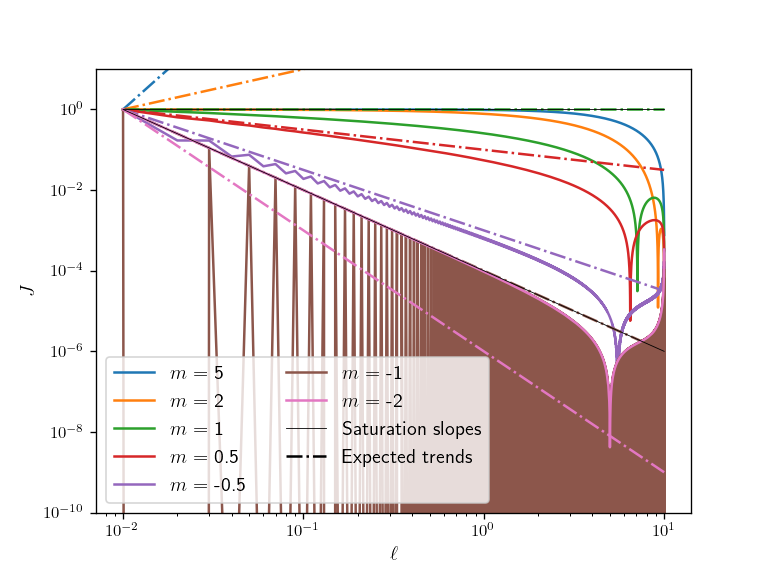
\includegraphics[width=\textwidth,trim = 0.5cm 0.5cm 2cm 2cm, clip]{./Mainmatter/Part_Appendix/images/sat_cor}
          \caption{\ensuremath{\mathcal{R} = <A'\cdot B + A\cdot B'>} }
          \label{fig:sat_corr}
      \end{subfigure}
      \hfill
      \begin{subfigure}[b]{0.496\textwidth}
          \centering
          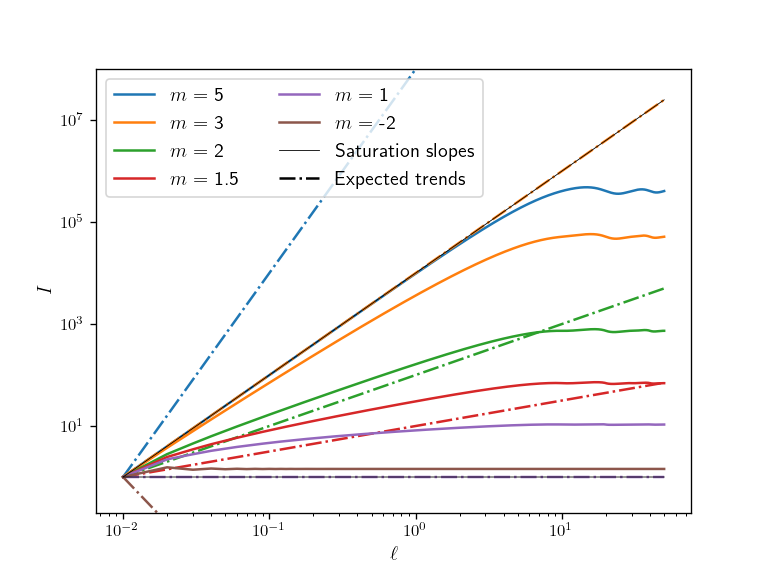
\includegraphics[width=\textwidth,trim = 0.5cm 0.5cm 2cm 2cm, clip]{./Mainmatter/Part_Appendix/images/sat_inc}
          \cprotect\caption{\ensuremath{\mathcal{S}=<\left(A'-A\right)\cdot\left(B'-B\right)>} }
          \label{fig:sat_inc}
      \end{subfigure}
         \cprotect\caption{Lignes pleines colorées : fonction de corrélation suivent la loi d'échelle spectrale de puissance \ensuremath{m}. Lignes discontinues colorées : tendance attendue pour chaque \ensuremath{m} si n'y pas de saturation mathématique. Lignes fines noires : tendance des saturations. }
        \label{fig:sat_trends}
  \end{figure}
 Ces tendances sont représentées sur la figure \figref{fig:sat_corr} pour $\mathcal{R}$ et \figref{fig:sat_inc} pour $\mathcal{S}$. On retrouve aussi la prédiction de \cite{cho_simulations_2009} pour les fonctions de corrélation de type $\mathcal{S}$ avec $A=B$. Cette prédiction est étendue ici à $A\neq B$ et $m<0$.  On s'attend donc à retrouver ce genre de saturations mathématiques dans nos simulations pour l'hyperdissipation qui se comporte tel que $m \ll -1$. L'équivalence nécessaire pour le passage de $\mathcal{R}$ à $\mathcal{S}$ en soustrayant à $\mathcal{R}$ sa valeur en $\ell = 0$ pour obtenir $\mathcal{S}$ est montrée sur la figure \figref{fig:sat_comp}.


  \begin{figure}
  \center
 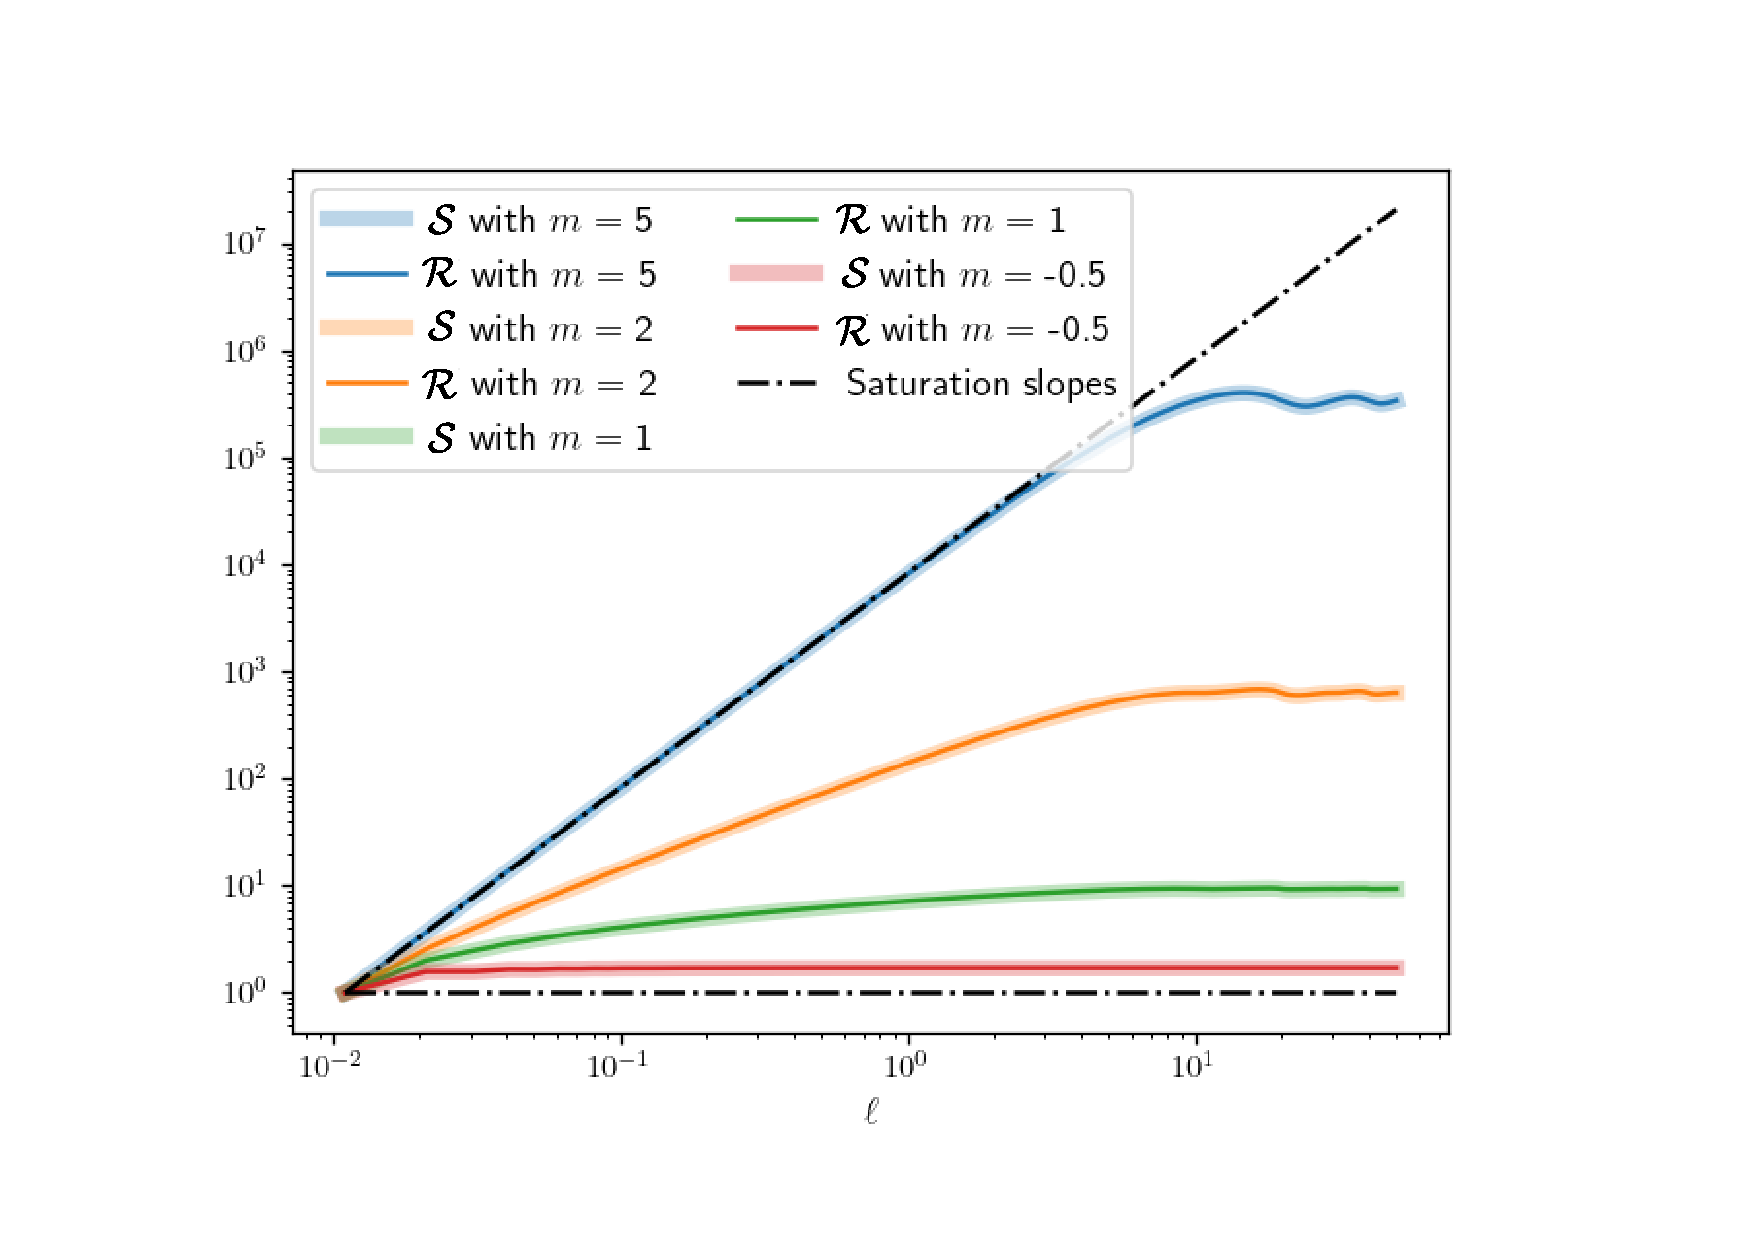
\includegraphics[width=0.5\textwidth,trim = 2cm 0.5cm 2cm 2cm, clip]{./Mainmatter/Part_Appendix/images/sat_comp_2}
 \cprotect\caption{Équivalence entre \ensuremath{\mathcal{S}} (lignes épaisses) et \ensuremath{2<A\cdot B> - \mathcal{R}} (lignes fines). Couleurs : \ensuremath{m}. Lignes discontinues : saturations. }
 \label{fig:sat_comp}
 \end{figure}
  
 Cette démonstration montre que le lien entre tendance spectrale et fonction de corrélation n'est pas évident. Quelques pincettes sont donc à prendre lorsque l'on veut interpréter les résultats des lois \cacro{KHM}, en particulier à travers l'hypothèse de séparation d'échelle. Ce n'est pas parce que le forçage n'est supposé agir qu'à grande échelle que sa contribution, $\varepsilon_F$, à la loi \cacro{KHM} tendra vers 0 aux autres échelles. Elle restera en effet constante. De même, en fonction de sa forme, incrémentale ou non, la contribution dissipative sera ou constante ou de pente $2$ ou $-2$. \cite{ferrand_multi-scale_2021} a proposé quelques méthodes afin de contourner ce problème dans le cas incompressible mais leur validité est questionnable dans le cas compressible. Comme on a pu le remarquer, une méthode simple peut aider à l'interprétation de ces contributions : regarder conjointement les lois \cacro{KHM} qui sont incrémentales et celles qui ne le sont pas. Si les fonctions de corrélation permettant de les obtenir sont bien choisies, il est très facile de passer de l'une à l'autre en soustrayant les valeurs obtenues en $\ell=0$. 
